\documentclass[12pt]{ctexart}
\usepackage{amsmath}
\usepackage{amsthm}
\usepackage{amssymb}
\usepackage{amsfonts}
% \usepackage{geometry}
\usepackage{graphicx}
\usepackage{bookmark}
\usepackage{tikz-cd}
% \usepackage{hyperref}

\theoremstyle{definition}
\newtheorem{theorem}{Def}[section]
\newtheorem{lemma}[theorem]{Lemma}
\theoremstyle{definition}
\newtheorem{definition}{定义}[section]
\newtheorem{thm}[definition]{定理}
\newtheorem{proposition}[definition]{性质}

\theoremstyle{plain} 
\newtheorem{exam}[definition]{Example}
\theoremstyle{remark}
\newtheorem{remark}[definition]{Remark}

\begin{document}
\title{作业}
\maketitle
\paragraph{1. } \(\{ \epsilon , \varnothing, \{ \varnothing \}\}\) 的幂集. 
\[
\{ 
	\{ \epsilon \} , \{ \varnothing \} , \{ \{ \varnothing \}\} ,
	\{ \epsilon , \varnothing  \},  \{ \epsilon , \{ \varnothing  \} \} , \{ \varnothing  , \{ \varnothing  \}\} , 
	\varnothing  , \{ \epsilon , \varnothing , \{ \varnothing  \} \} 
\}
\]

\paragraph{2. } 见图~\ref{fig:2}
\begin{figure}[h]
	\centering
	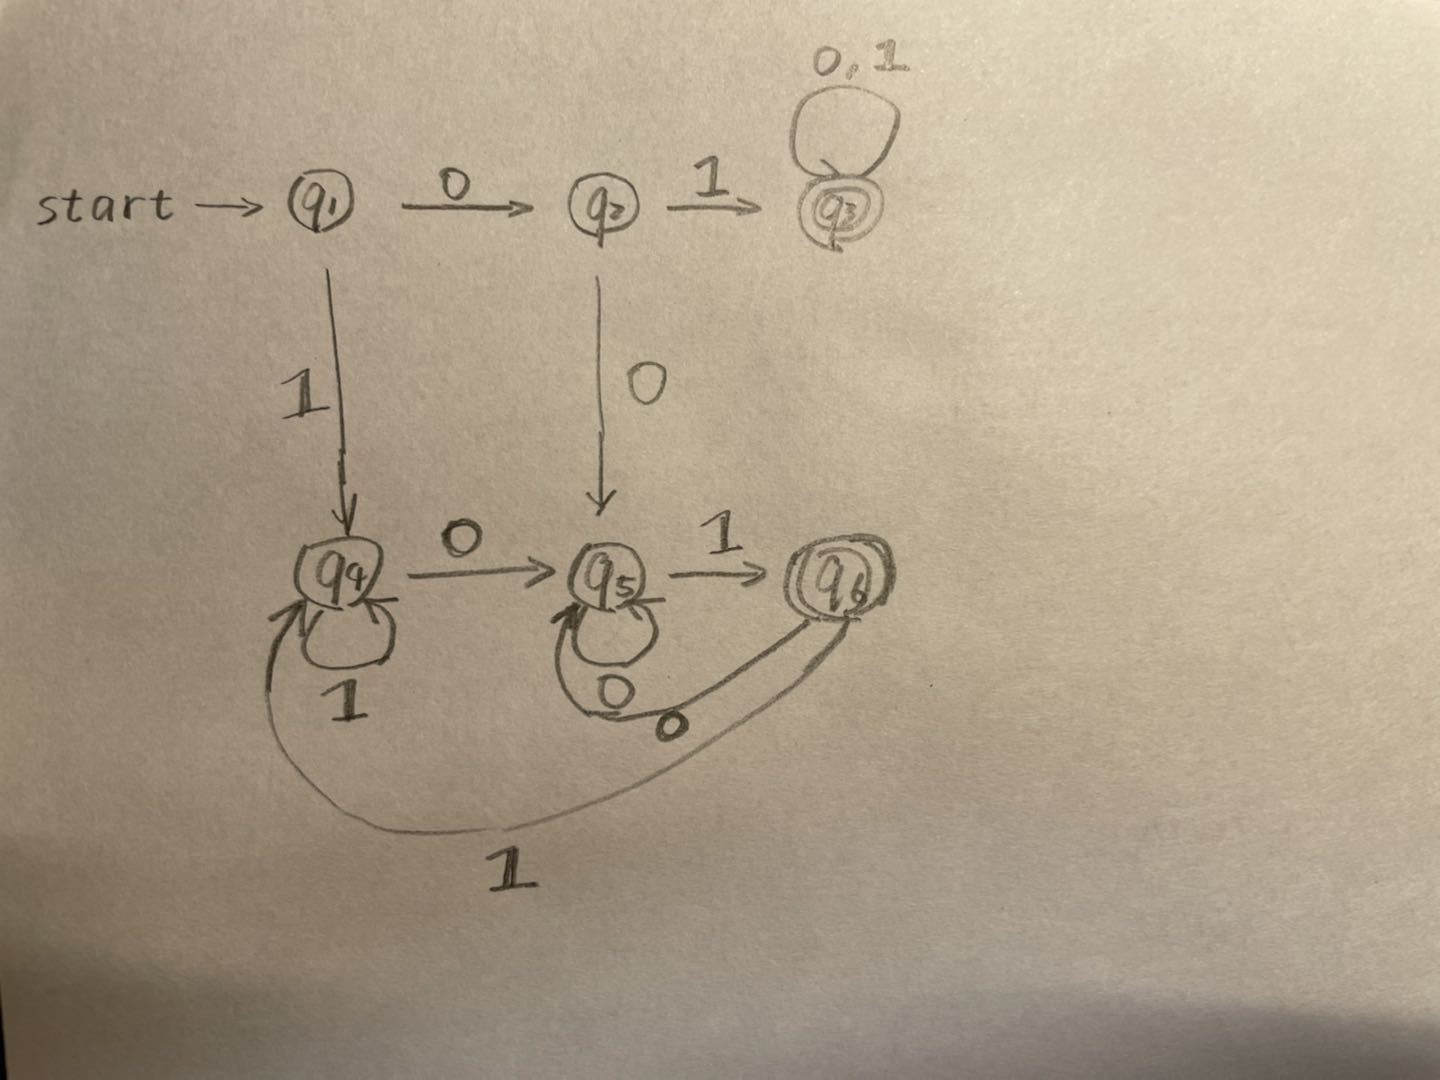
\includegraphics[width=\linewidth]{hw01_2.jpg}
	\caption{题2}\label{fig:2}
\end{figure}

\paragraph{3. } 见图~\ref{fig:3}
\begin{figure}[h]
	\centering
	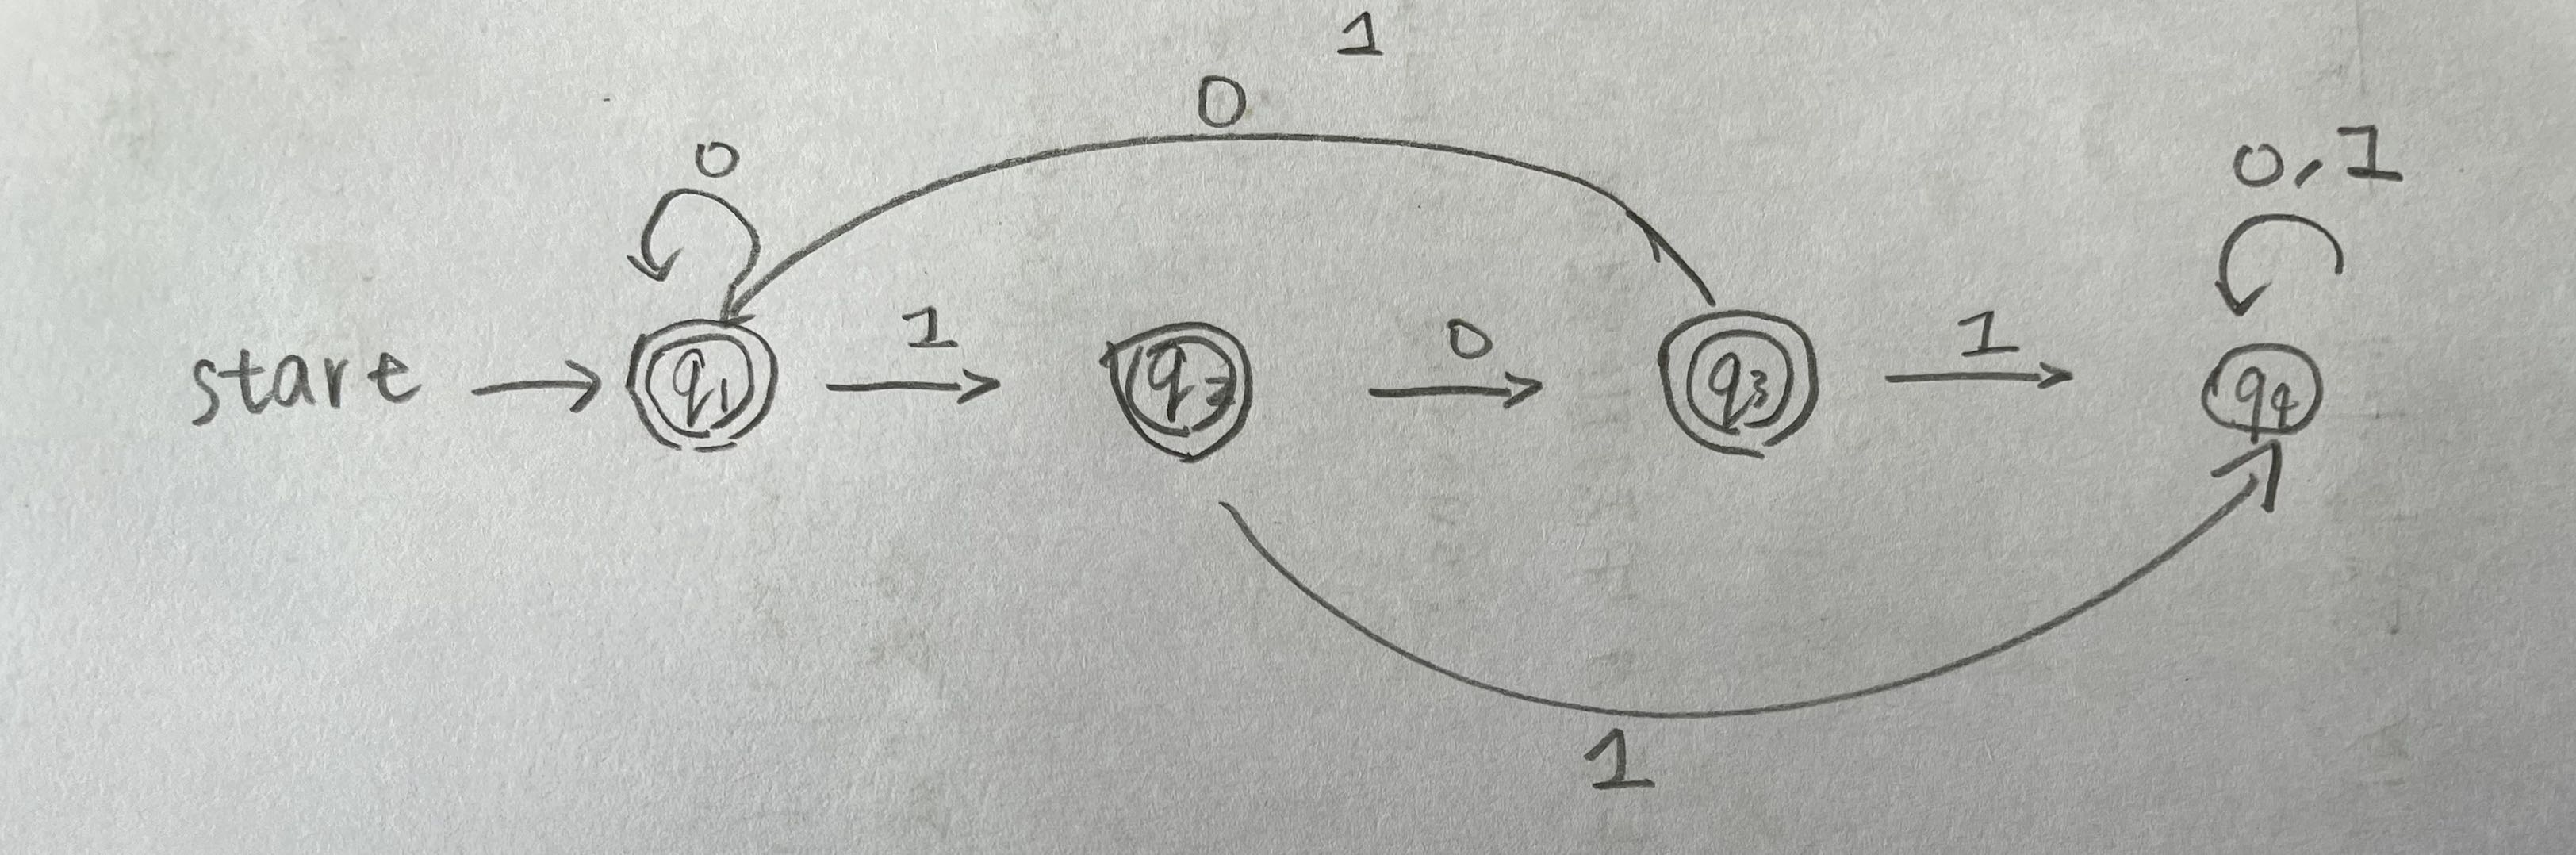
\includegraphics[width=\linewidth]{hw01_3.jpg}
	\caption{题3}\label{fig:3}
\end{figure}

\paragraph{4. (a)}
% \begin{equation*}
% 	\big( (1 (11 ) ^{*} 0 (0 (11) ^{*}0 ) ^{*} + 0(00) ^{*} 1 (1 (00) ^{*} 1 ) ^{*} ) (1 (11 ) ^{*} 0 (0 (11) ^{*}0 ) ^{*} + 0(00) ^{*} 1 (1 (00) ^{*} 1 ) ^{*} ) \big) ^{*}
% \end{equation*}
% 
% 
% 设 \((1 (11 ) ^{*} 0 (0 (11) ^{*} 0) ^{*} + 0(00) ^{*} 1 (1 (00) ^{*} 1 ) ^{*} )\) 为 \(w\). 则正则语言为 \( (ww ) ^{*}\)

% 设 \( 1 (11)^{*} 0 (0 (11)^{*} ) ^{*} \) 为 \(a\), \( 0 (00) ^{*} 1 (00) ^{*} 1 ) ^{*}\) 为 \(b\), 则 \(w = a + b\)

\[
	( 00 + 11 ) ^{ *} + ((00 + 11 )^{*} ( 01 + 10 )( 00 + 11 ) ^{*} (01 + 10 ) ( 00 + 11) ^{*}  )^{*}
\]



\paragraph{4. (b)}
见图~\ref{fig:42}. 答案为
\(
	0^{*}(1 1 ^{*} 00 ) ^{*}
\).
\begin{figure}[h]
	\centering
	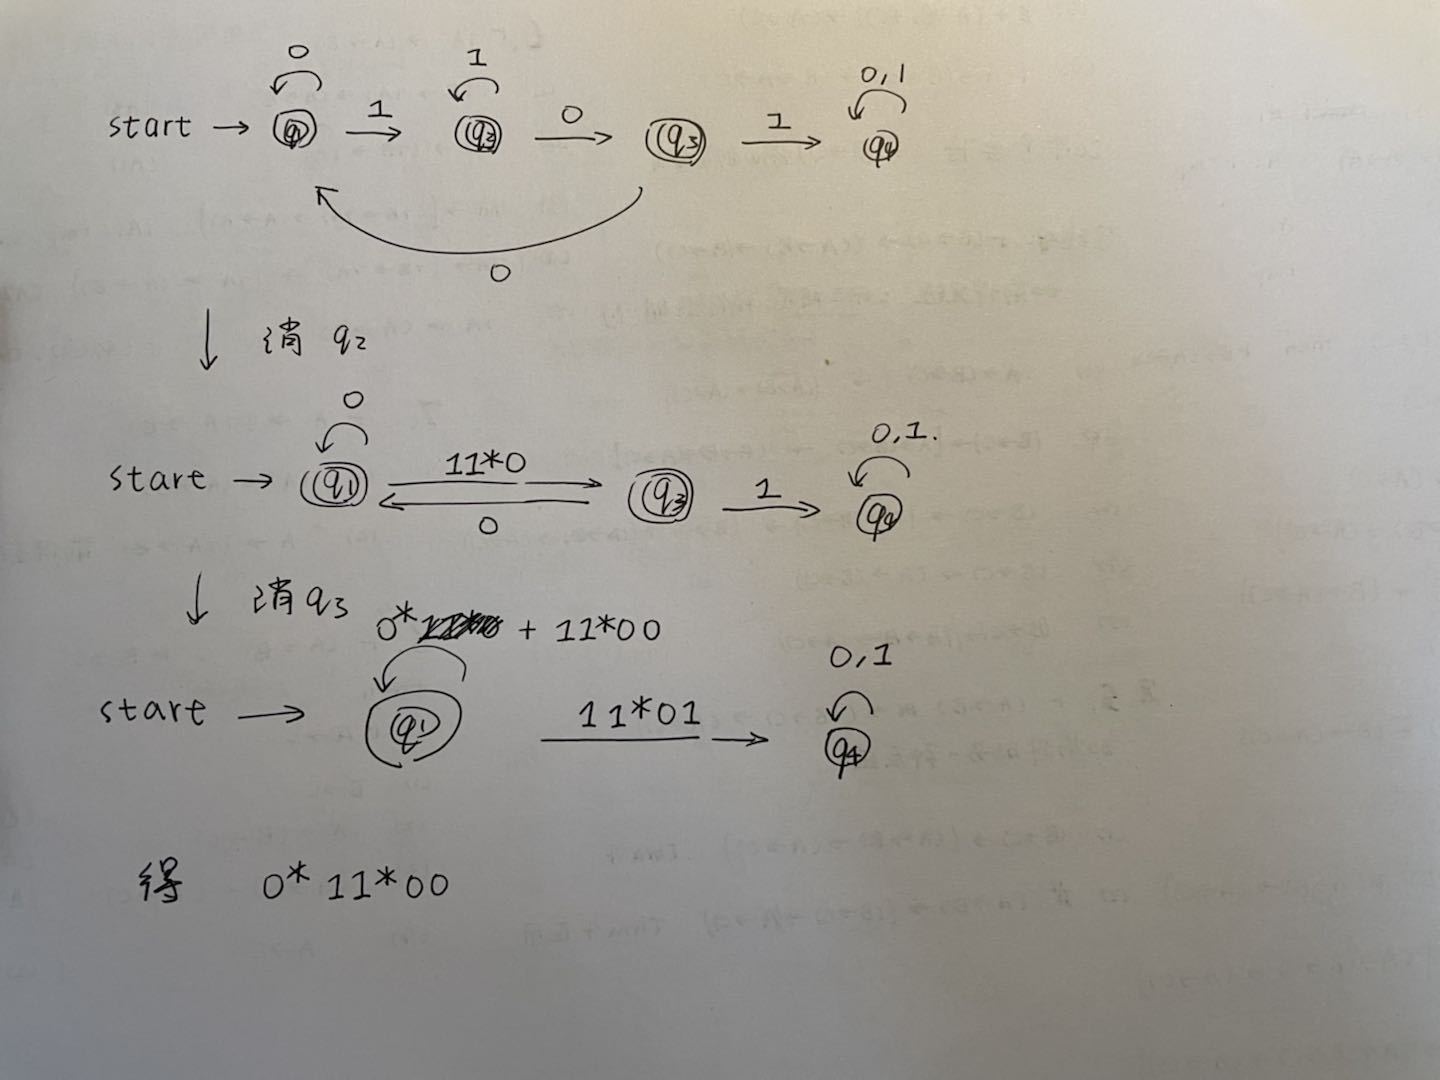
\includegraphics[width=\linewidth]{hw01_42.jpg}
	\caption{题4.(b)}\label{fig:42}
\end{figure}


% \begin{figure}
% \centering
% \begin{tabular}{c|c|c|c} \hline 
% 	 &0&1&2\\\hline
% 	0& & & \\\hline
% 	1& & & \\\hline
% 	2& & & \\\hline  
% \end{tabular}
% \end{figure}

\begin{figure}
\centering
\begin{tabular}{c|c|c|c} \hline 
	 &0&1&2\\\hline
	0&1&0& \\\hline
	1& &0&1\\\hline
	2&1&0 & \\\hline  
\end{tabular}\caption{k=\(-1\)}\label{tab:k=-1}
\end{figure}

\begin{figure}
\centering
\begin{tabular}{c|c|c|c} \hline 
	 &0&1&2\\\hline
	0&1*&1*0& \\\hline
	1&&0&1\\\hline
	2&11*&0+11*0&\\\hline  
\end{tabular}\caption{k=0}\label{tab:k=0}
\end{figure}
\begin{figure}
\centering
\begin{tabular}{c|c|c|c} \hline 
	 &0&1&2\\\hline
	0&1*&1*00*&1*00*1\\\hline
	1&&0*&0*1 \\\hline
	2&11*&(0+11*0)0*&(0+11*0)0*1\\\hline  
\end{tabular}\caption{k=1}\label{tab:k=1}
\end{figure}

\paragraph{5.} 
递归的过程见图~\ref{tab:k=-1}, 图~\ref{tab:k=0}, 图~\ref{tab:k=1},
\(0+ 11 * 0 \) 化简为 \(1 ^{*}0\). 
故对应的正则语言应该为 \(1 ^{*} 0 0 ^{*} 1(1^{*}0 0 ^{*} 1 )^{*}\)


\end{document}
